\documentclass[11pt,a4paper]{article}

\usepackage[utf8]{inputenc}
\usepackage[english]{babel}
\usepackage{amsmath}
\usepackage{amsfonts}
\usepackage{amssymb}
\usepackage{graphicx}
\usepackage[left=3cm,right=3cm,top=3cm,bottom=3cm]{geometry}

\usepackage{hyperref}
\usepackage{caption}
\usepackage{subcaption}
\usepackage{mathtools}

\usepackage{listings}
\usepackage{color}

\lstset{
	language=Scala,
	keywordstyle=\color{blue},
	frame = single
}

\author{Hugo Kapp 227942}
\title{Semester project report}

\newcommand{\scala}[1]{\textsf{#1}}
\newcommand{\nir}[1]{\texttt{#1}}

\begin{document}

\maketitle

\section{Introduction}

We explain in this report all that was done during this semester project : the goals, the ideas and results achieved. We give in this section insights about why this project is important, as well as the ground we start with. We then give the details of each optimization that is implemented, and pointers to their correctness.

\subsection{Motivation}

In recent compilers, compilation speed is an issue. This is particularly important in Scala compilers, because the richness of the language is hard to resolved automatically. The process is therefore slower than for other languages. For ScalaNative, this problem is worsened by the long compilation time of LLVM, which is relatively slow when applied to big files. Because there is no dynamic linking in ScalaNative, all symbols and definitions that can be reached during the execution of the program are statically linked during compilation. This leads to a very big program that needs to go through the whole compilation pipeline, even for very small input programs.

All of this makes the ScalaNative compiler very slow, and produces huge executables.

\subsection{Goal}

The goal of this project is therefore to reduce the amount of code worked with, through various optimizations. We could let the LLVM compiler take care of all of this, as it has a very efficient optimization pipeline. The idea here is to take advantage of the domain-specific knowledge we have, before it is lost due to primitives lowering to LLVM. On top of that, having less code to perform the passes on should speed up the compilation.

The only goal here is code reduction, and not execution speed. Any reduction in the final size of the executable, as well as compilation or execution speed-up, in totally incidental, but will still be noted.

\subsection{The ScalaNative compiler}

Before we start explaining the various optimizations implemented and their impact, we first need to talk a little bit about the compiler organization and specific. Only what is necessary is explained here, and kept abstract. For more details on the compiler, please refer to the documentation in \cite{nativedoc}.

\subsection*{Compiler organization}

The compiler is organized as a classic pipeline consisting of a sequence of \scala{Pass}.  For this project, we only add passes to the compilation pipeline, which will alter the current form of the code.

\subsubsection*{Native Intermediate Representation}

Scala Native uses its own intermediate representation (IR), called \textit{Native Intermediate Representation} and abbreviated NIR.

It is in SSA form, which stands for \textit{Static Single Assignment}. This means that variables have only one static definition in the program, which can be performed multiple times during execution. Different values can then be merged to define a new variable, using the concept of $\phi$-functions that can be found in the litterature (see \cite{ssabook}). In NIR, classic $\phi$-functions are replaced by arguments passed to each basic block.

The instruction set of NIR is composed of a subset of LLVM operations, with the same semantics, plus some high-level constructs coming from Scala. The latter are lowered during the compilation process to be expressed in terms of LLVM instructions.

Further details about NIR can be found in \cite{nirdoc}.

\section{Global Value Numbering}

The first optimization implementend is called Global Value Numbering, and sometimes abbreviated GVN.

\subsection{Idea}

The idea is taken directly from \cite{ssabook}, which also provides a proof of correctness. The general idea is to reuse the result of computations that were already made in the past, which makes GVN a redundancy elimination optimzation. To be able to do that, two conditions need to be met :

\begin{enumerate}
\item The two computations yield the same result in all cases, and there is no side-effect
\item In all possible paths of the control flow, the result we want to reuse has been computed before the location we want to reuse it at
\end{enumerate}

The first condition is very simple to understand, but the second might seem more complex. It can be explained using the example in Figure \ref{fig:gvn}. In \ref{fig:gvn1}, the computation \scala{a + 1} is not necessarily done when we reach the definition of \scala{c}. In \ref{fig:gvn2}, the result has already been computed when we reach the definition for \scala{b}, so we can avoid the re-computation of \scala{a + 1}.

\begin{figure}[h]
	\begin{subfigure}{0.5\textwidth}
		\begin{lstlisting}
if (...) {
  val b = a + 1
  ...
}
val c = a + 1
		\end{lstlisting}
		\caption{Unreduceable code}
		\label{fig:gvn1}
	\end{subfigure}
	\quad
	\begin{subfigure}{0.5\textwidth}
		\begin{lstlisting}
val c = a + 1
if (...) {
  val b = a + 1
  // val b = c
  ...
}
		\end{lstlisting}
		\caption{Reduceable code}
		\label{fig:gvn2}
	\end{subfigure}
	\caption{GVN examples}
	\label{fig:gvn}
\end{figure}

\subsection{Value Numbering}

Following its name, GVN uses value numbering to achieve the first condition. This is opposed to syntactic redundancy, where we consider that two expressions yield the same result only if they are written the same way (modulo the commutativity of operations).

In value numbering, each variable in the program has a hash value associated to it. We call the function that gives these hashes $h$. The hash value for variable $v$ is then given by $h(v)$. This value is computed using the defining operation for $v$, and the hash value for each of its operand. Note that this only works on programs that are in SSA form, like the NIR, because we need a single definition for each variable.

For example, say we have \nir{\%b = \%a + 1}. Then $h(\nir{\%b}) = h(\nir{\%a + 1}) = agg(\nir{+}, h(\nir{\%a}), h(\nir{1}))$. The aggregation function used ($agg$) is any hashing function.

Bootstrapping is done by giving each input variable a value that depend on its name. Constants are give a hash that depends on their value.

\subsection{Dominator tree}

To check for the second condition discussed earlier, we use the concept of dominator tree, also discussed in the SSA book \cite{ssabook}. From this very book, we get the following definition for domination :
\newline
A basic block $n_1$ \textit{dominates} basic block $n_2$ if every path in the control flow graph from the entry point to $n_2$ includes $n_1$. By convention, every basic block dominates itself.

In other words, $n_2$ is dominated by $n_1$ if we have to go through $n_1$ before going to $n_2$. Thus, if $v_1$ is defined in block $n_1$ and $v_2$ is defined in block $n_2$, and $n_1$ dominates $n_2$, then we know that the value of $v_1$ has been computed when we reach the definition of $v_2$. Note that this only holds if $n_1 \neq n_2$, but if it is the case, then it is trivial to check that $v_1$ is indeed defined before $v_2$.

We use this to build the dominator tree, which gives, for each block in the CFG, the set of blocks that dominate it. This allows us to easily check if the value of a variable $v$ can be used at a given point $p$ in the program, by verifying that $p$'s basic block is dominated by the block in which $v$ is defined.

\subsection{Algorithm}

Using both parts, we can then easily check which variables always have the same value, and reduce the ones computed later. The algorithm is as follows : \newline
For each instruction:
\begin{enumerate}
\item Compute the value for $v$, $h(v)$, using the values for its operands
\item For each variable $w$ that has the same value :
	\begin{enumerate}
	\item Check if the definitions for $v$ and $w$ match
	\item Check if the value of $w$ can be reused at $v$
	\item If both conditions are verified, then replace $v$ by $w$
	\end{enumerate}
\end{enumerate}

\subsection{Implementation}

Here we give a few details on the implementation on the described technique of Global Value Numbering.

First, we build the dominator tree by doing a single pass through the CFG. For each block $n_i$, the blocks dominating it is the set $D_i = \{i\} \cup \left( \bigcap\limits_{j \in pred(i)} D_j \right)$, where $pred(i)$ gives the set of predecessors to the block $n_i$ in the CFG. When the CFG contains loops, we need to do a fixpoint to find the correct domination set.

We use the \textsf{Murmur3} hash function, from the scala standard library (\scala{scala.util.hashing.MurmurHash3}). This provides good and very fast hashes, which is useful because we don't need cryptographic-level hashing. We take 32 bits hashes because it is convenient (it allows us to use the \scala{hashCode} function whenever possible), and is enough not to produce collisions (false positives, discussed later).

Even with hashing done correctly, we still need to define what it means for two variables to have the same definition. This is done in a recursive manner, using the following rules :
\newline
Two variables $a$ and $b$ are \textit{deep equal} if:
\begin{enumerate}
\item $a$ and $b$ have the same name (they are indeed the same variable)
\item or their respective definitions match, i.e. they use the same operation, and their operands are \textit{deep equal}
\end{enumerate}

Having defined all of this, we just follow the algorithm sketched above, building the dominator tree before going through the code. Note that, when a variable $b$ is found to be replaceable by the value of another variable $a$, we use a simple NIR instruction \nir{copy}, which avoids having to replace $a$ by $b$ everywhere (\nir{copy} instructions are simplified later in the pipeline).

\section{Control-flow optimizations}

We discuss in this section various optimizations that are aimed at simplifying the control-flow graph.

\subsection{Unit simplification}

\subsubsection*{Problem}

In Scala, every code block has a value. This is very useful in general, but sometimes the value is not used. Nevertheless, it has to be accounted for by the compiler, that the value of this block might be used later in the future. This is especially true for if-then-else blocks, where the value is usually not important. In such cases, the types of the last instruction of the said blocks rarely match, or match with unit (with assignment variables for example).

% the case is actually if alone (no else) !

In this case, the Scala Native compiler still needs a way to merge the outcomes of these code blocks, and does so by having the next basic block have a parameter of type \scala{Unit}, where the two branches give their own output value. This is shown in Figure \ref{fig:cfc}. This is not necessary, as we know that \scala{Unit} is the type that has only one value (the \scala{Unit} object).

\subsubsection*{SimplifyUnit}

To solve this problem, we add a very simple pass to the compiler, called \scala{SimplifyUnit}. Its job is very simple : whenever a variable of type \scala{Unit} is used (either as an operand, or given as a parameter to a block or function), it is replaced by the actual value \scala{Unit}.

This is helpful because the LLVM compiler can not simplify all of these variables later, because it doesn't know that the type \scala{Unit} only has one value. But this alone wouldn't be enough.

\subsubsection*{Dead parameters elimination}

Simplifying the unit usage is a nice thing, but it still leaves a complicated CFG, with a lot of unused block parameters. Even if the parameter variable with type \scala{Unit} was indeed used in the block, its use gets replaced by the value \scala{Unit}. Therefore, all block parameters with type \scala{Unit} can be removed.

We can actually generalize this by adding to the normal \scala{DeadCodeElimination} phase a simple analysis on the block parameters on top of the normal variables. This simplifies the CFG a lot, and makes it more readable.

Note that these improvements do not reduce the code size by themselves (not in terms of code lines at least), but allows for further optimizations in the other passes, and increases the optimization potential of LLVM as well.

\subsection{Control-flow chains}

\subsubsection*{Problem}

The original CFG produced by the compiler is very simple. For any control-flow branching, it produces a "diamond", which is the result of the left branch and right branch dissociating, then merging in the next shared portion of the code. But in many cases, this is not necessary.

For example, take the code in Figure \ref{fig:cfc} and its (simple) CFG. Because there is no "else" part to the "if", we could already jump to the block \nir{\%src.5} without going through \nir{\%src.4} if the condition is not met.
% This goal CFG is shown in \ref{fig:cfc:cfg2}.

\begin{figure}[h]
	\begin{subfigure}{0.5\textwidth}
		\begin{lstlisting}
if (...) {
  println(..)
}
// no else
		\end{lstlisting}
		%\caption{Simple example code}
		%\label{fig:cfccode}
	\end{subfigure}
	\quad
	\begin{subfigure}{0.5\textwidth}
		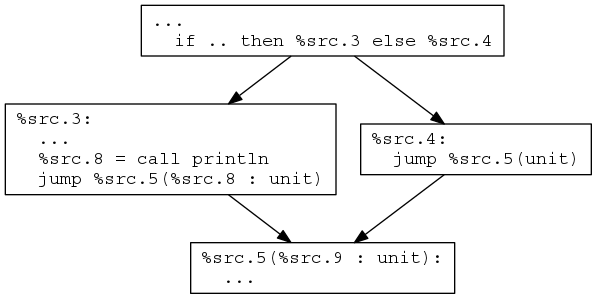
\includegraphics[width=\textwidth]{images/cfc-cfg1.png}
		%\caption{Reduceable code}
		%\label{fig:cfccfg1}
	\end{subfigure}
	\caption{A simple code example, and its corresponding CFG}
	\label{fig:cfc}
\end{figure}

\subsubsection*{CfChainsSimplification}

To solve the kind of problems explained above, we add a new pass to the compiler, called \scala{CfChainsSimplification}. Its goal is to simplify the control flow using global CFG informations, and in particular to solve these simple control-flow chains, where a block is only comprised of a single control-flow instruction. We use the following rules for simplification :

$$ \frac{\nir{\%a(\%b..): Cf}}{\nir{jump \%a(\%c..)} \longrightarrow \nir{Cf} \  | \  \{\nir{\%b..} \rightarrow \nir{\%c..}\}} $$

$$ \nir{if true then \%a(\%b..) else \%c(\%d..)} \longrightarrow \nir{jump \%a(\%b..)} $$

$$ \nir{if false then \%a(\%b..) else \%c(\%d..)} \longrightarrow \nir{jump \%c(\%d..)} $$

$$ \frac{\nir{jump \%a(\%b..)} \longrightarrow^* \nir{jump \%a'(\%b'..)} \quad \nir{jump \%c(\%d..)} \longrightarrow^* \nir{jump \%c'(\%d'..)}}{\nir{if \%e then \%a(\%b..) else \%c(\%d..)} \longrightarrow \nir{if \%e then \%a'(\%b'..) else \%c'(\%d'..)}} $$

$$ \nir{switch \%a \{ default: \%b \} } \longrightarrow \nir{jump \%b} $$

$$ \frac{\nir{\%a = \%b}_i}{\nir{switch \%a \{ cases \%b..: \%c.. ; default: \%d \} } \longrightarrow \nir{jump \%c}_i} $$

$$ \frac{\nir{jump \%c}_i \longrightarrow^* \nir{jump \%c'}_i \quad \nir{jump \%d} \longrightarrow^* \nir{jump \%d'}}{\splitfrac{\nir{switch \%a \{ cases \%b..: \%c.. ; default: \%d \} }}{\longrightarrow \nir{switch \%a \{ cases \%b..: \%c'.. ; default: \%d \} }}} $$

Where \nir{Cf} is any single control-flow instruction.

The pass does fixpoint iterations on each control-flow instruction, following the rules above, until convergence for this instruction has been reached. This is particularly useful when the control flow chains are rather long, and static information is carried along (for example a \nir{jump true} that jumps to an \nir{if} can directly be reduced).

\subsection{Merging basic blocks}

\subsubsection*{Idea}

A very simple control-flow simplification is the one that reduces unnecessary basic blocks. The conditions for a block $n_1$ to be removed is that is has only a single predecessor in the CFG $n_p$, and $n_p$ must have a single successor in the CFG. In this case, we can merge the two blocks into one, because we know the control flow will always go to $n_1$ at the end of $n_p$, and $n_1$ is not used anywhere else.

This is an easy way to reduce the CFG and the number of branching that appear in the code. On top of that, because the parameters of the fused block now have known values, additional optimizations may trigger, simplifying the code further.

\subsubsection*{BasicBlocksFusion}

For this implementation, we add a new pass called \scala{BasicBlocksFusion}, which fuses together blocks that satisfy the aforementioned conditions.

\subsection{Reducing block parameters}

\subsubsection*{Problem}

Even after the passes described above have been executed, there is still information that can be extracted from the CFG and be made explicit. We talk here about block parameters that are always supplied the same argument. We can simplify these by removing the said parameter, and replacing it by its supplied value. This simplifies the CFG, because blocks have less parameters, and makes their value explicit, allowing further optimizations to trigger.

\subsubsection*{BlockParamReduction}

Once again, we add a new pass, called \scala{BlockParamReduction}. First, it gathers the argument values that are supplied to each block parameter in the CFG. Then, parameter \nir{\%a} is removed if the set of supplied values has a single value, not counting the recursive value \nir{\%a}. We then remove the arguments from the branching locations. All of this can be done in three passes : one to build the CFG, one to gather the arguments, and one to simplify the branching and the parameters.

\section{Static evaluation}

We discuss here various static evaluation and pattern-based optimizations.

\subsection{Canonicalization}

% inspired by LLVM

\subsubsection*{Goal}

Because the partial evaluation and instruction combine passes are pattern-based, and some of these pattterns depend on the presence of static values (i.e. not variables), we perform canonicalization first. The goal of canonicalization is to simplify the writing of patterns, by ensuring an invariant on their location. We use here the same convention as in the LLVM compiler, and say that any static value that can be moved, is moved to the right operand. This means we only move operands for commutative operations.

\subsubsection*{Canonicalization}

The \scala{Canonicalization} pass is very simple. For each instruction, if it is commutative and has a static operand, then it is moved to the right-hand side.

This only makes sense to perform on binary operations. The only such instructions in NIR are arithmetic, logical and comparison operators. All of these are also LLVM instruction, with the same semantics. Because LLVM has a very efficient optimization pipeline, the goal here is not to do better than the underlying compiler, but to extract simple statically known information that might be useful for the other optimization passes (which use domain-specific knowledge).

Note that we do not modify instructions that manipulate floats (these are explicit instructions), because float handling is too complicated for the purpose of this project. We therefore let all float-instructions optimization to LLVM. We prefer safety over mis-optimization.

\subsection{Constant folding}

\subsubsection*{Idea}

Constant folding is very simple. It basically emulates the run-time output of each instruction that has all its operands statically known. We can therefore propagate the knowledge we have further in the code.

This is simple, but needs to capture perfectly the semantics of each operation. Most of them can easily be performed in Scala, but some of the low-level instructions may be hard to express in such a high-level language.

Here again, we do not do anything with float instructions, to make sure we keep the semantics of the original program intact.

\subsubsection*{ConstantFolding}

We add a pass called \scala{ConstantFolding}. Because it needs all its operands to be static, it is not dependent on the \scala{Canonicalization} pass. This pass is only concerned with low-level instructions, because high-level instructions with static values are optimized in their own lowering pass. This is then a trivial pass, but special care has to be taken to follow the semantics of the LLVM operators.

\subsection{Partial evaluation}

\subsubsection*{Idea}

The idea of partial evaluation is to use simple rules to simplify single instructions that have some static information. An example would be to say that $a \times 0$ can always be replaced by the value $0$, irrespective of the value of $a$.

Such optimization passes are a set of patterns which, when they apply to the current input, need to simplify the code in some way or another. The code reduction is an obvious target, but not necessarily the best. One can easily devise a (potentially abritrary) total ordering on the set of instructions, and say that the lower instructions are simpler. In this case, reducing the code size, or bringing an operation down in the ordering are acceptable simplifications.

Making sure that each pattern actually simplifies the code is important. It may provide a  very easy check for useless patterns, but also ensures that a fixpoint method will always converge.

\subsubsection*{PartialEvaluation}

We add yet another pass to the compiler, called \scala{PartialEvaluation}. It is a list of single-instructions patterns that all simplify the code. The ordering over the instructions can easily be devised, and is relatively intuitive, but is not detailed here. Because using a \nir{copy} operation is effectively reducing the code size, it is quite obvious that the \nir{copy} instruction is at the bottom of this ordering.

\subsection{Instruction combine}

\subsubsection*{Idea}

The idea for this optimization is inspired by the LLVM pass called \scala{InstCombine} \cite{llvm}. Relatively close to partial evaluation, this pass goes further and simplifies patterns that use knowledge about variable definitions. It is therefore able to capture patterns that span mutliple instructions.

\subsubsection*{InstCombine}

We add a pass called \scala{InstCombine}. Its role is to simplify multi-instructions patterns in the code. Very close to partial evaluation, it is however distinct, because it deals with much more involved patterns, and doesn't require the operands to have statically known values. It uses the operation defining its variable operands to perform optimizations.

\begin{figure}[h]
	\begin{subfigure}{0.5\textwidth}
		\begin{lstlisting}
%a = ...
%b = xor %a, true
if %b then %c else %d
		\end{lstlisting}
		\caption{Raw code}
	\end{subfigure}
	\quad
	\begin{subfigure}{0.5\textwidth}
		\begin{lstlisting}
%a = ...
%b = xor %a, true
if %a then %d else %c
		\end{lstlisting}
		\caption{Optimized code}
	\end{subfigure}
	\caption{A code pattern simplifiable by instruction combine}
	\label{fig:ic}
\end{figure}

An example that occurs a lot in the produced code is shown in Figure \ref{fig:ic}. The \nir{xor} with the value \nir{true} is used to negate a boolean value, as LLVM doesn't have a negation opertator. This code is the result of a simple \scala{if (!a)} expression in the original scala code. We can avoid computing the intermediate value \nir{\%b} by simply switching the branching destinations. Note that the optimized version of the code does not get rid of the definition for \nir{\%b}. This is because it could be used somewhere else in the code, although this is unlikely. Anyway, it will be cleaned up by the dead code elimination pass if possible.

The criteria for reducing code is thus more complex than the one used in the last section. Here, on top of reducing instructions to simpler ones, we can also reduce the number of variable used. This may lead to some variables being reomved by DCE, which eventually reduces the code size. 


% need a note on passes placement

% add examples everywhere !

\section{Results}

We discuss in this section the impact the optimizations mentioned in the above sections had.

\subsection{Methodology}

We here describe the methodology used to measure the impact of the optimization, as well as the metrics used : how they are computed, and how they can be interpreted.

\subsubsection{Code base compilation}

\label{codebase}

The linker of the Scala Native compiler gathers all the code that is potentially reachable from the main program given. Because it is hard to produce a program that reaches the maximum number of classes and methods possible, we bypass the linker. We create a routine that gathers all symbols (classes and methods) in the entire code base, and run the compilation passes on this code.

The code base is the product of all the code that is pre-compiled and kept in \texttt{.nir} files. It is composed of the entire Scala library, a specific Scala Native library, as well as the parts of the Java library that have been re-implemented in Scala for the purpose of Scala Native. We also have some other programs and benchmarks.

The entire code base described here contains, as of January 3rd, 2017, 5195 compiled files, for a total of 588'295 lines of NIR code. However, because the Scala library has some dependency on the Java library, and that the latter is not complete, some of the files have to be disabled. This leads to a valid codebase of 210'228 lines of NIR code. This will give a reasonable approximation of the impact the added pass have on general purpose code, due to the size and diversity of goals for the different code sources.

\subsubsection{Metrics}

We detail here the various metrics used to measure the performance achieved by the implemented optimizations.

\subsubsection*{Raw code reduction}

The first, and most obvious metric, is the raw code reduction. Mostly shown as a percentage of line reduction, it is sometimes used as the raw number of lines removed by the various optimization phases.

\subsubsection*{Optimizeable code reduction}

An extension of the previous criterion is called \textit{optimizeable} code reduction.

The problem with the raw code reduction is that it doesn't take into account what could have been changed, and what has to be fixed. For example, all the global definitions that have to be there (NIR declares classes and traits separately from the methods they define). All of these cannot be reduced. On top of that, each method needs to have a first line of declaration, an entry block label, at least one control flow instruction, and a closing brace.

Using this knowledge, we define the optimizeable code of some program as :

$$ opt(p) = \sum\limits_{m \in methods(p)} size(m) - 4 $$

This gives us a metric that takes into account how reduceable the code actually is.

\subsubsection*{Touched methods}

One other way to think about the changes the optimizations added have on the codebase is to see how many methods it affects, and out of these, what is the code reduction. This may give more insight on the effect had.

% add std-dev for code reduction out of touched methods

\subsection{Observed results}

We show here the results observed on the code base described in \ref{codebase}. We talk mostly about code reduction, but also show briefly the variations in executable size, compilation time and execution time.

\subsubsection{Code reduction}



\subsubsection{Other impacts}

% executable size difference !

\section{Future work}


\section{Conclusion}


\begin{thebibliography}{9}

   \bibitem{nativedoc} Scala Native documentation \newline \url{http://scala-native.readthedocs.io}

	\bibitem{nirdoc} NIR documentation \newline \url{http://scala-native.readthedocs.io/en/latest/contrib/nir.html}
	
	\bibitem{ssabook} SSA book
	
	\bibitem{llvm} LLVM compiler passes \newline \url{http://llvm.org/docs/Passes.html}

\end{thebibliography}


\end{document}